
\begin{figure}[t!]
	\captionsetup{justification=justified, singlelinecheck=false, width=1\textwidth}
    \caption{Evento regional natural registrado em 2023-16-06 11:22:00 (UTC) nas proximidades da cidade de Iguape – SP. A) Localização do evento (círculo vermelho maior) em relação à estação SP7 (círculo vermelho menor) e B) Forma de onda do evento registrada na estação SP7.}
    \begin{mdframed}[
        linecolor=black,
        linewidth=1pt,
        roundcorner=10pt,
    ]
    \begin{center}
    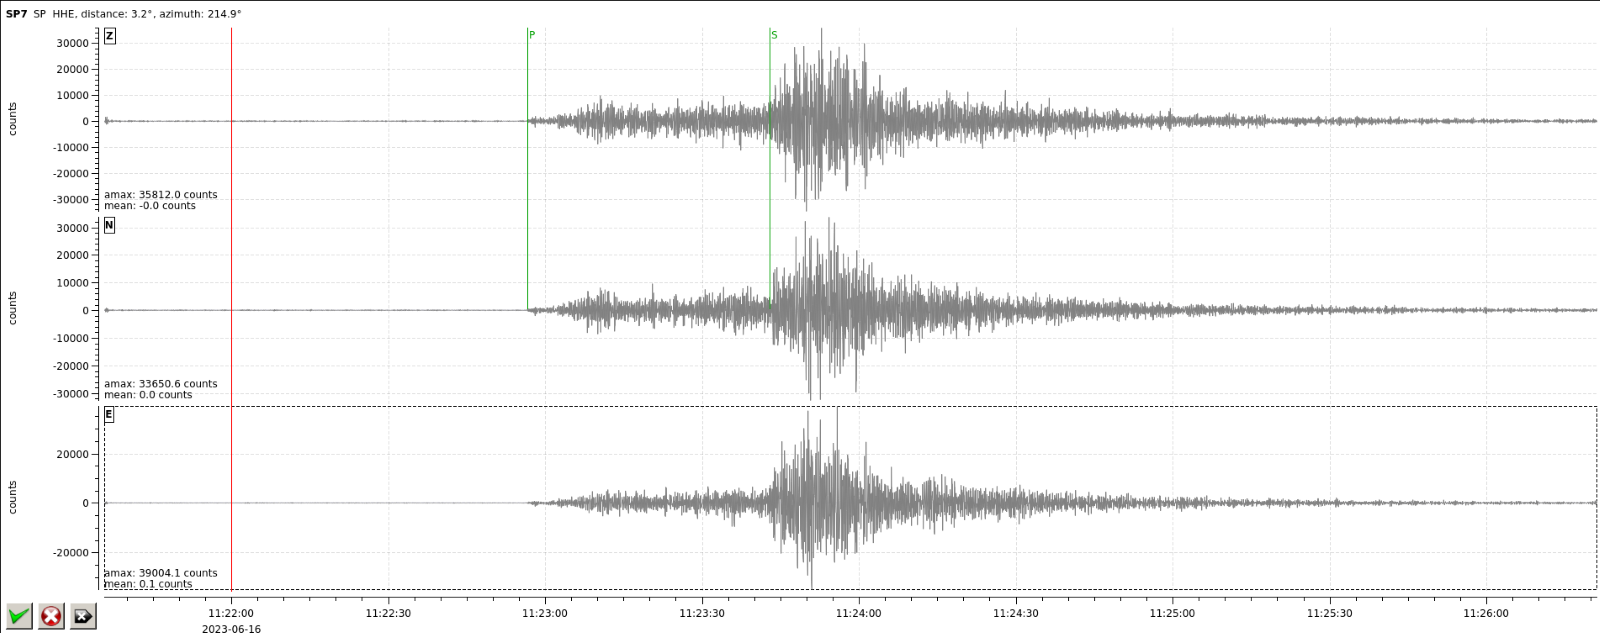
\includegraphics[width=0.8\textwidth]{./relatorio/figuras/evento_regional.png}
    \end{center}
    \end{mdframed}
    \caption*{Fonte: IPT}
\end{figure}
